%%%%%%%%%%%%%%%%%%%%%%%%%%%%%%%%%%%%%%%%%
% Beamer Presentation
% LaTeX Template
% Version 1.0 (10/11/12)
%
% This template has been downloaded from:
% http://www.LaTeXTemplates.com
%
% License:
% CC BY-NC-SA 3.0 (http://creativecommons.org/licenses/by-nc-sa/3.0/)
%
%%%%%%%%%%%%%%%%%%%%%%%%%%%%%%%%%%%%%%%%%

%----------------------------------------------------------------------------------------
%	PACKAGES AND THEMES
%----------------------------------------------------------------------------------------

\documentclass{beamer}

\mode<presentation> {

% The Beamer class comes with a number of default slide themes
% which change the colors and layouts of slides. Below this is a list
% of all the themes, uncomment each in turn to see what they look like.

%\usetheme{default}
%\usetheme{AnnArbor}
%\usetheme{Antibes}
%\usetheme{Bergen}
%\usetheme{Berkeley}
%\usetheme{Berlin}
%\usetheme{Boadilla}
%\usetheme{CambridgeUS}
%\usetheme{Copenhagen}
%\usetheme{Darmstadt}
%\usetheme{Dresden}
%\usetheme{Frankfurt}
%\usetheme{Goettingen}
%\usetheme{Hannover}
%\usetheme{Ilmenau}
%\usetheme{JuanLesPins}
%\usetheme{Luebeck}
\usetheme{Madrid}
%\usetheme{Malmoe}
%\usetheme{Marburg}
%\usetheme{Montpellier}
%\usetheme{PaloAlto}
%\usetheme{Pittsburgh}
%\usetheme{Rochester}
%\usetheme{Singapore}
%\usetheme{Szeged}
%\usetheme{Warsaw}

% As well as themes, the Beamer class has a number of color themes
% for any slide theme. Uncomment each of these in turn to see how it
% changes the colors of your current slide theme.

%\usecolortheme{albatross}
%\usecolortheme{beaver}
%\usecolortheme{beetle}
%\usecolortheme{crane}
%\usecolortheme{dolphin}
%\usecolortheme{dove}
%\usecolortheme{fly}
%\usecolortheme{lily}
%\usecolortheme{orchid}
%\usecolortheme{rose}
%\usecolortheme{seagull}
%\usecolortheme{seahorse}
%\usecolortheme{whale}
%\usecolortheme{wolverine}

%\setbeamertemplate{footline} % To remove the footer line in all slides uncomment this line
%\setbeamertemplate{footline}[page number] % To replace the footer line in all slides with a simple slide count uncomment this line

%\setbeamertemplate{navigation symbols}{} % To remove the navigation symbols from the bottom of all slides uncomment this line
}

\usepackage{graphicx} % Allows including images
\usepackage{booktabs} % Allows the use of \toprule, \midrule and \bottomrule in tables

%----------------------------------------------------------------------------------------
%	TITLE PAGE
%----------------------------------------------------------------------------------------

\title[Short title]{Efimov Physics -- The Three-Body Problem} % The short title appears at the bottom of every slide, the full title is only on the title page

\author{Kajsa-My Blomdahl} % Your name
\institute[SU] % Your institution as it will appear on the bottom of every slide, may be shorthand to save space
{
Stockholms Universitet \\ % Your institution for the title page
\medskip
\textit{kajsamy.blomdahl@fysik.su.se} % Your email address
}
\date{\today} % Date, can be changed to a custom date

\begin{document}

\begin{frame}
\titlepage % Print the title page as the first slide
\end{frame}

%----------------------------------------------------------------------------------------
%	PRESENTATION SLIDES
%----------------------------------------------------------------------------------------

\begin{frame}
\frametitle{The Peculiar Efimov Effect}
\begin{itemize}
\item A quantum effect
\item Resonant 2-body forces can give rise to a series of bound energy levels in 3-particle systems
\item When the two-body s-wave scattering length $a \rightarrow \pm\infty$ the $\#$ of bound states is infinite
\item  $\#$ of 3-body bound states is \textit{reduced} as the two-body interaction is made more attractive
\item Emerge irrespective of the nature of the 2-body forces and can \textit{in principle} be observed in all quantum mechanical systems. 
\end{itemize}
\end{frame}

%------------------------------------------------

\begin{frame}
\frametitle{Scattering Length}
\begin{itemize}
	\item The 2-body $s$-wave scattering length describes the strength of the interparticle interaction. Definition:
	\begin{equation}
	a = \lim_{k \to 0} -\frac{\tan\delta_0(k)}{k}
	\end{equation}
	\item Negative scattering lengths correspond to an attractive effective interaction
	\item Positive scattering lengths correspond to a repulsive effective interaction
\end{itemize}
\end{frame}

\begin{frame}
\frametitle{Solving The 3-body Problem: Step 1, Jacobi Coordinates}
\begin{figure}
\centering
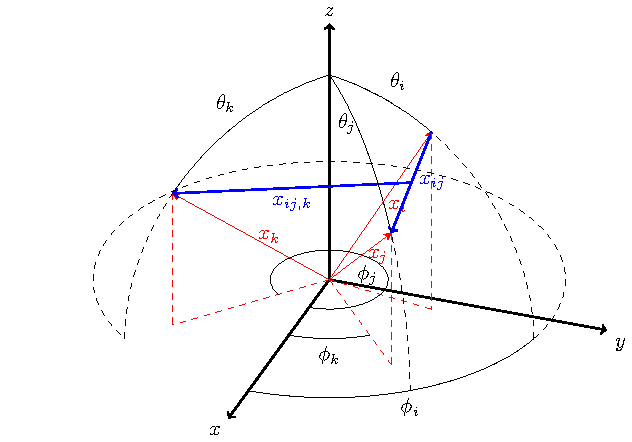
\includegraphics[width=0.7\linewidth]{img01.pdf}
\caption{Spatial positions of three particles.}
\end{figure}
\end{frame}

\begin{frame}
\frametitle{The Model Potential}
\begin{equation}
v(r) = d\cosh^{-2}{(r/r_0)},
\end{equation}
\end{frame}

\begin{frame}
\frametitle{$a>0$}
\begin{figure}
	\begin{figure}
		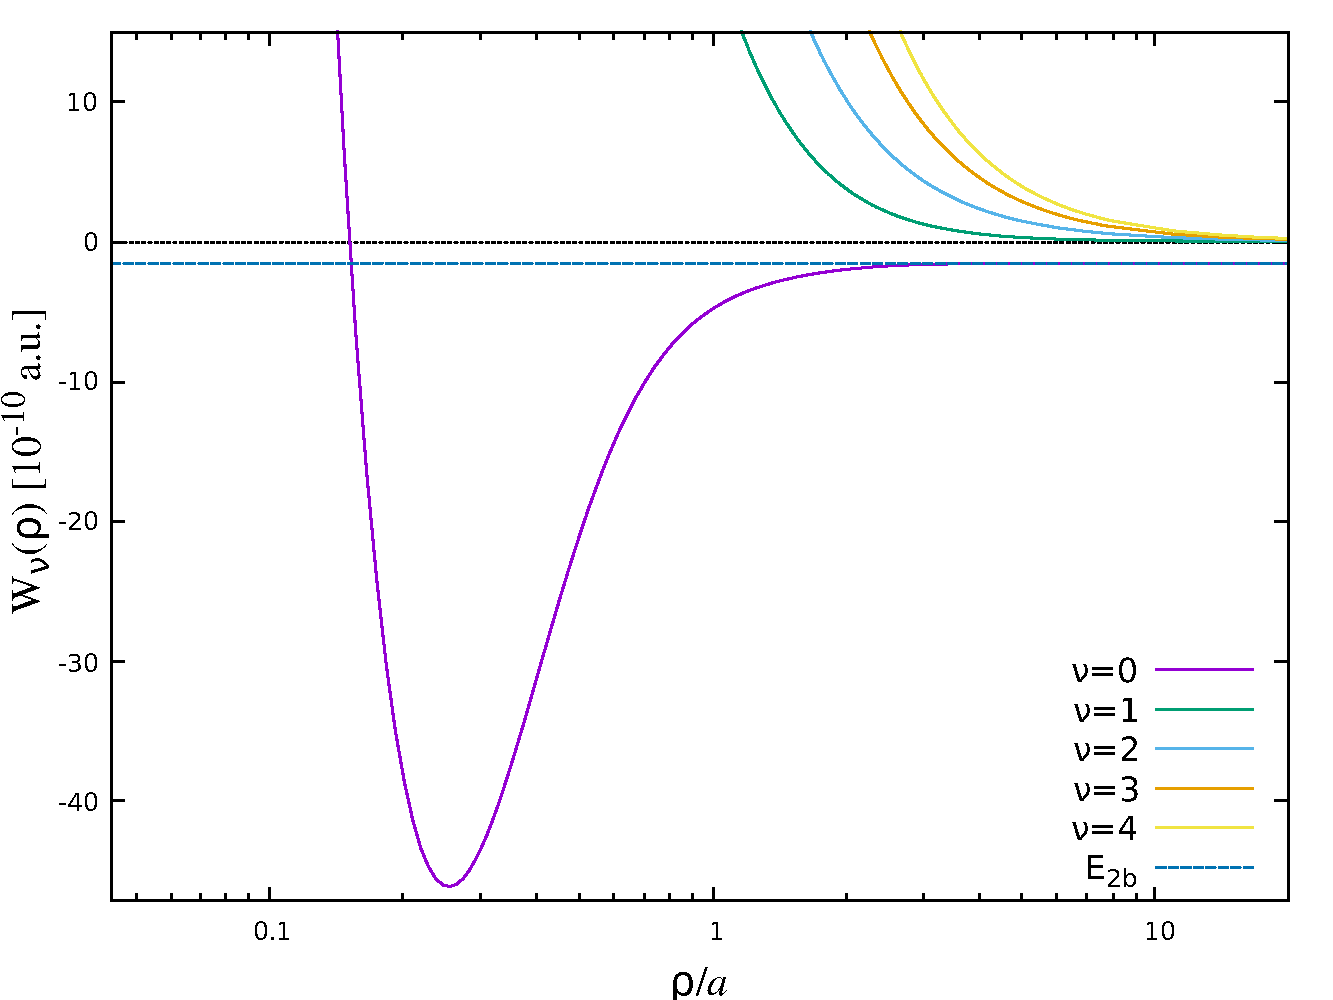
\includegraphics[width=0.8\linewidth]{Wpos.pdf}
	\end{figure}
\end{figure}
\end{frame}

\begin{frame}
\frametitle{$a<0$}
\begin{figure}
	\begin{figure}
		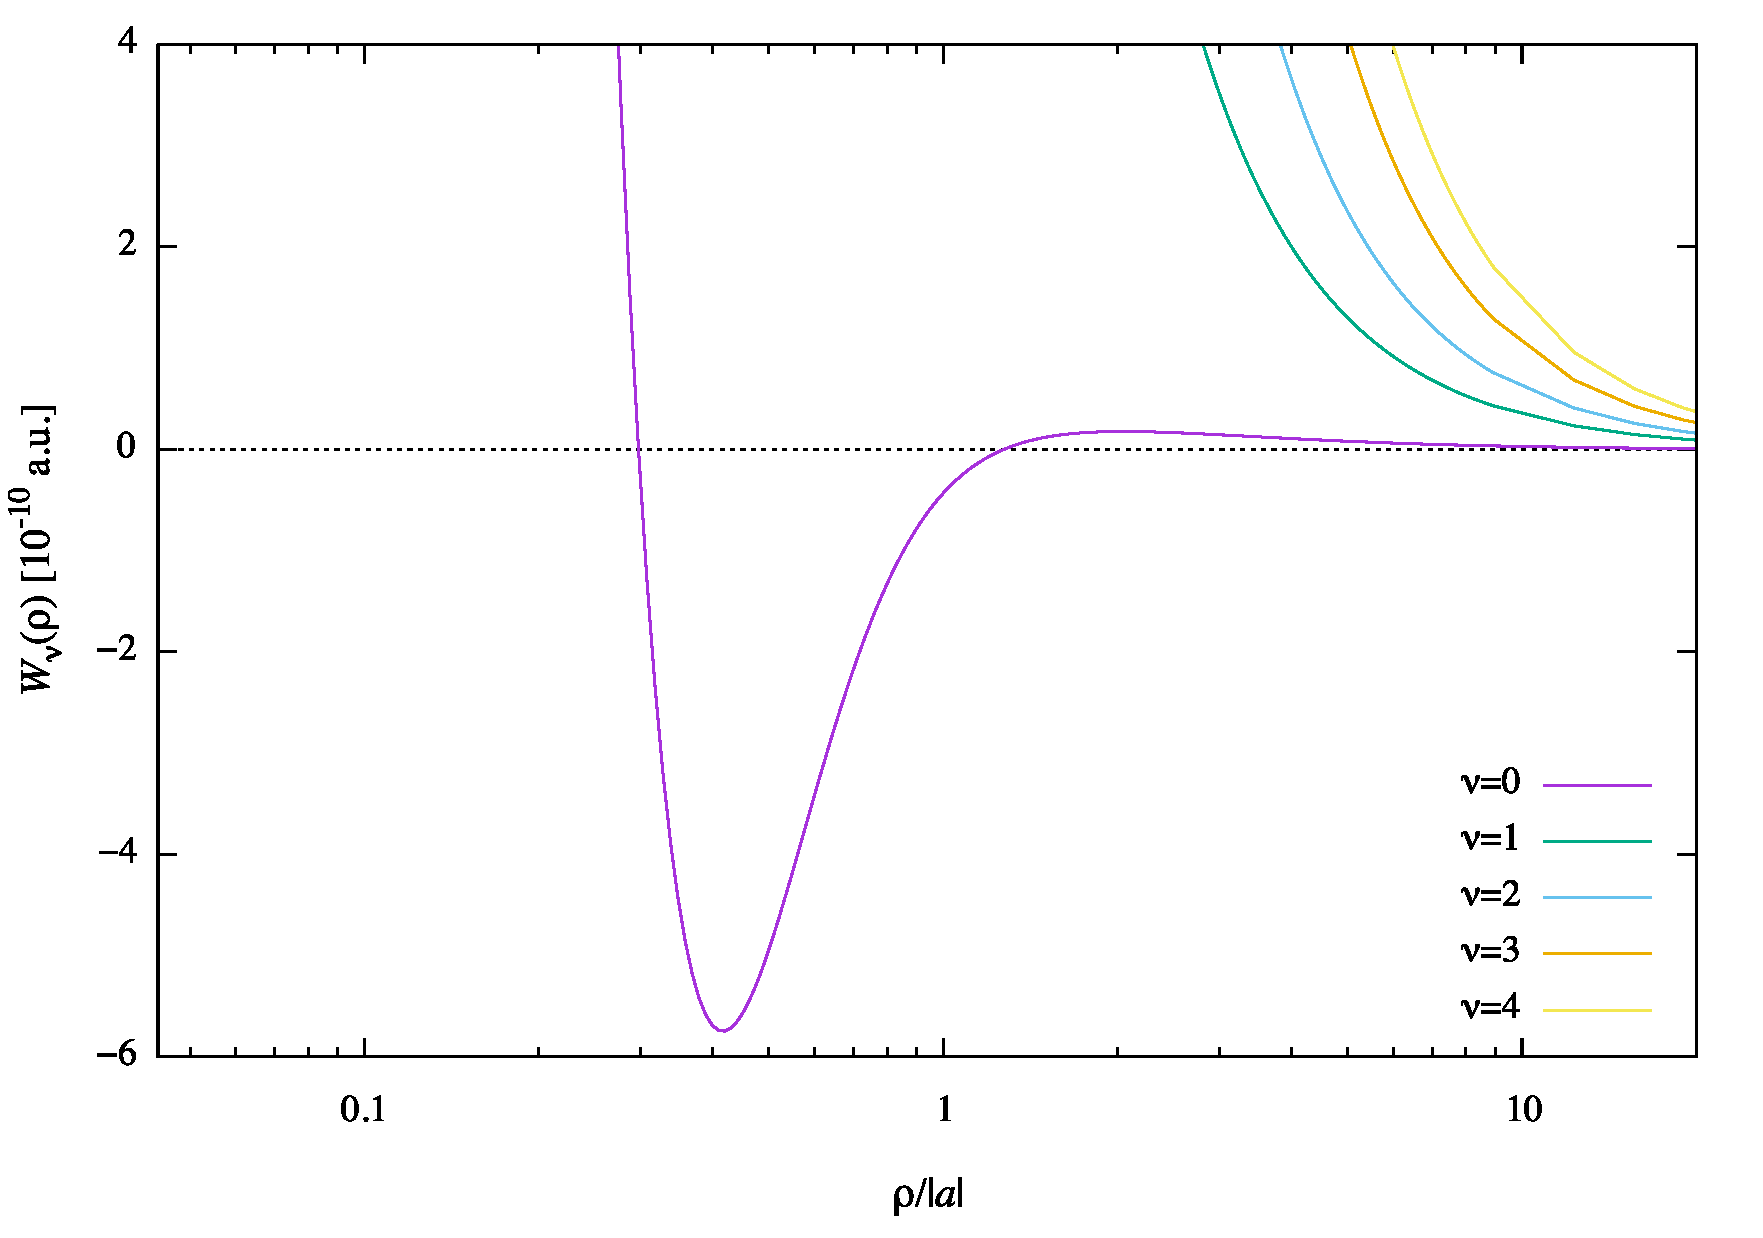
\includegraphics[width=0.8\linewidth]{Wneg.pdf}
	\end{figure}
\end{figure}
\end{frame}

%------------------------------------------------

\begin{frame}
\frametitle{$a \rightarrow \pm \infty$, $-s_0^2 (\simeq -1.0125$ for $J=0^+$ states)}
\begin{figure}
	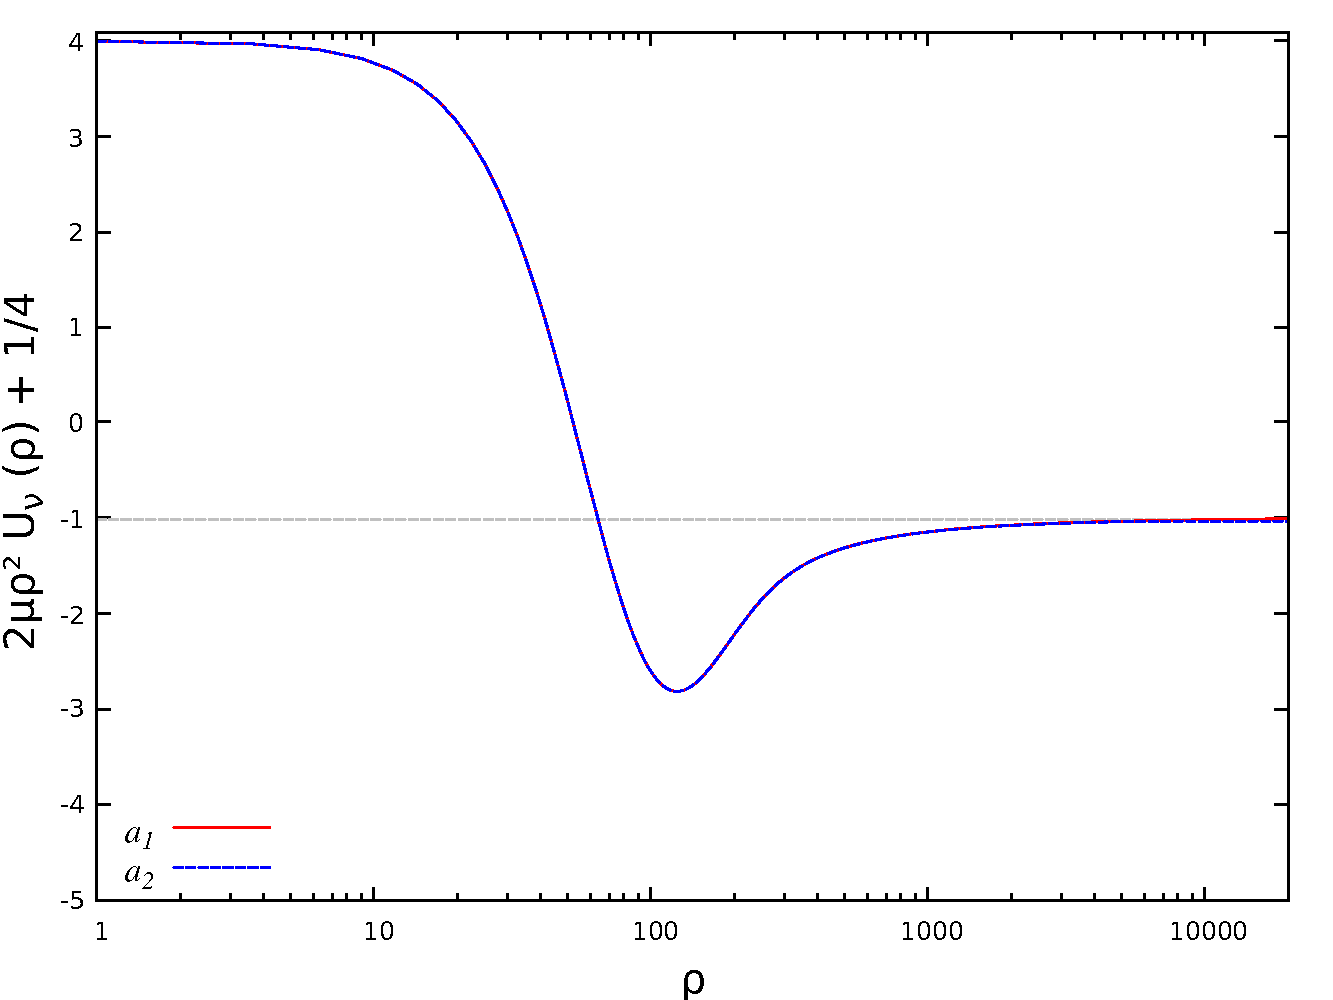
\includegraphics[width=0.8\linewidth]{infty.pdf}
\end{figure}
\end{frame}

\begin{frame}
\frametitle{$a >0$}
\begin{figure}
	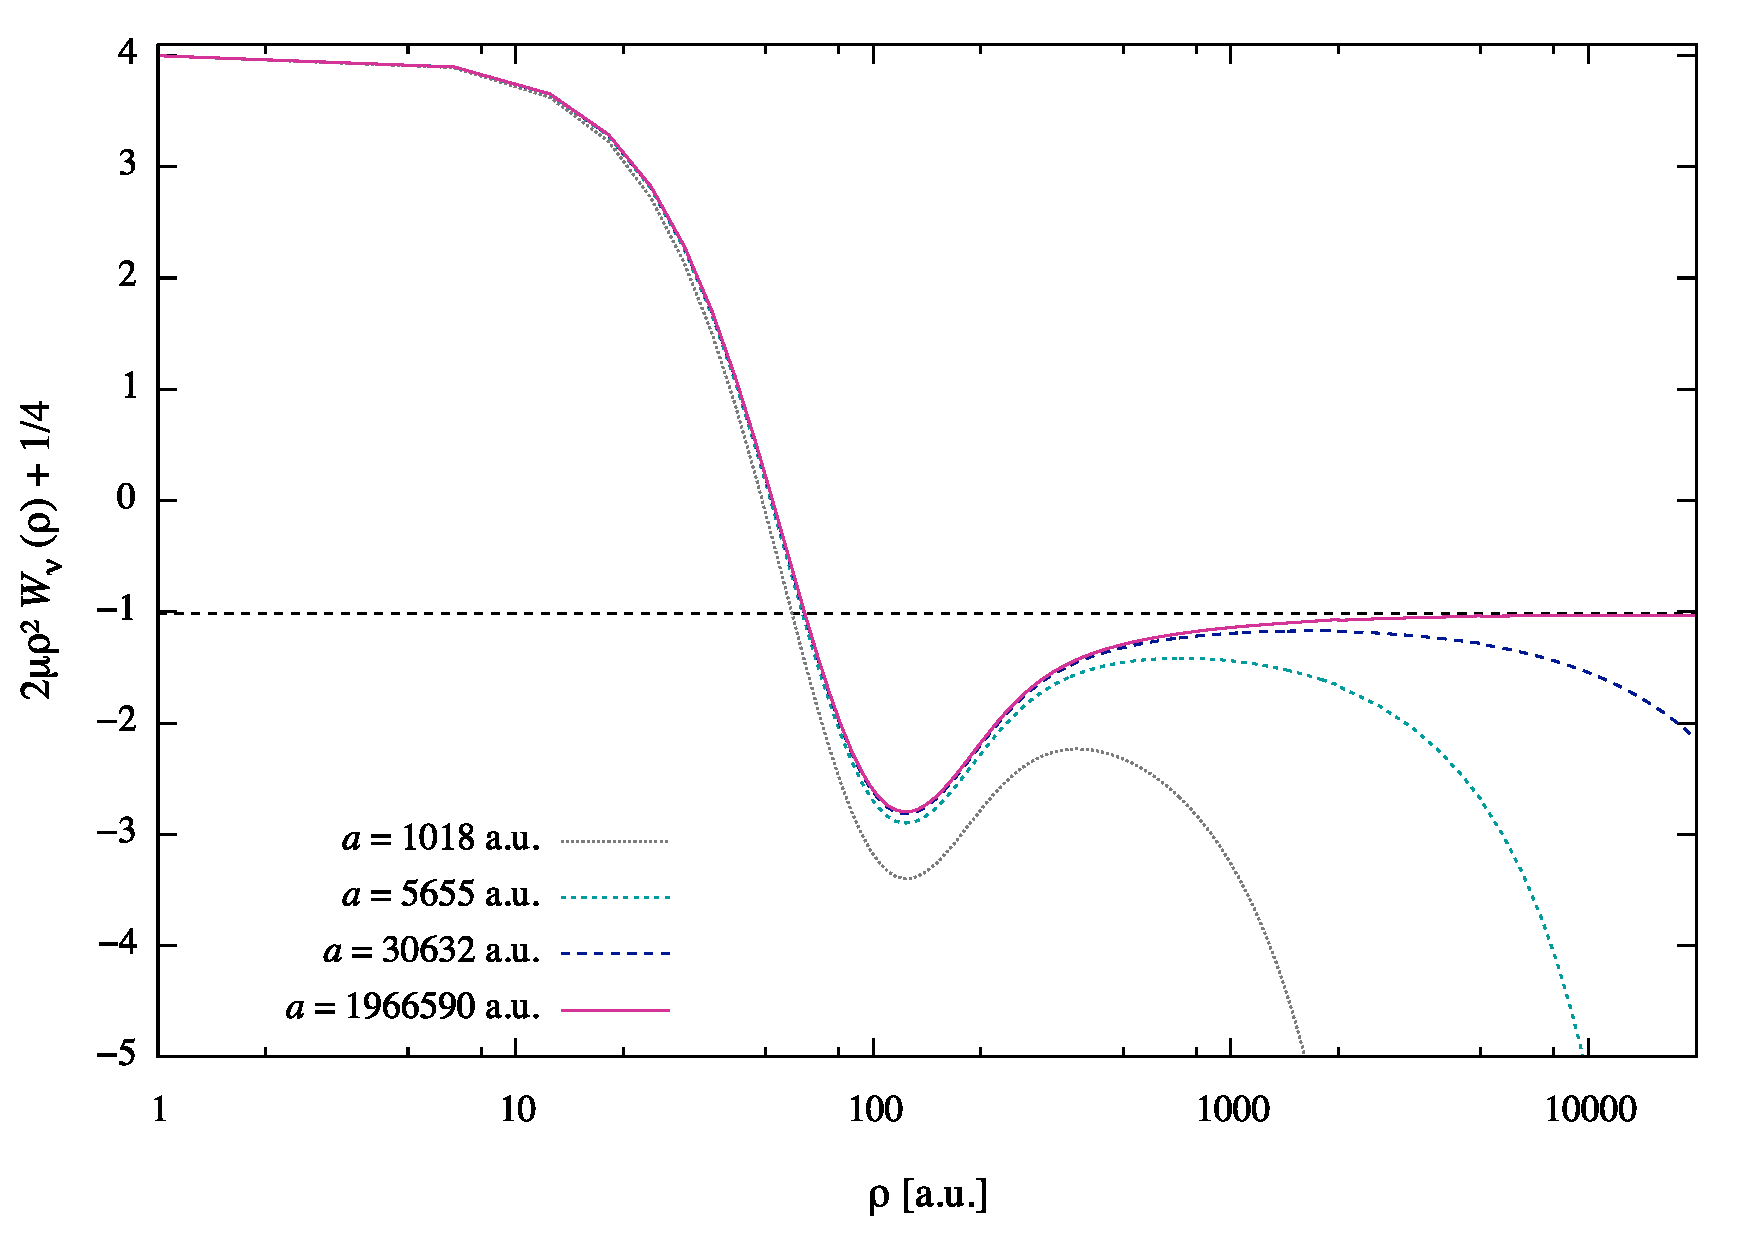
\includegraphics[width=0.8\linewidth]{finite_positive_a.pdf}
\end{figure}
\end{frame}

\begin{frame}
\frametitle{$a>0$}
\begin{figure}
	\begin{figure}
		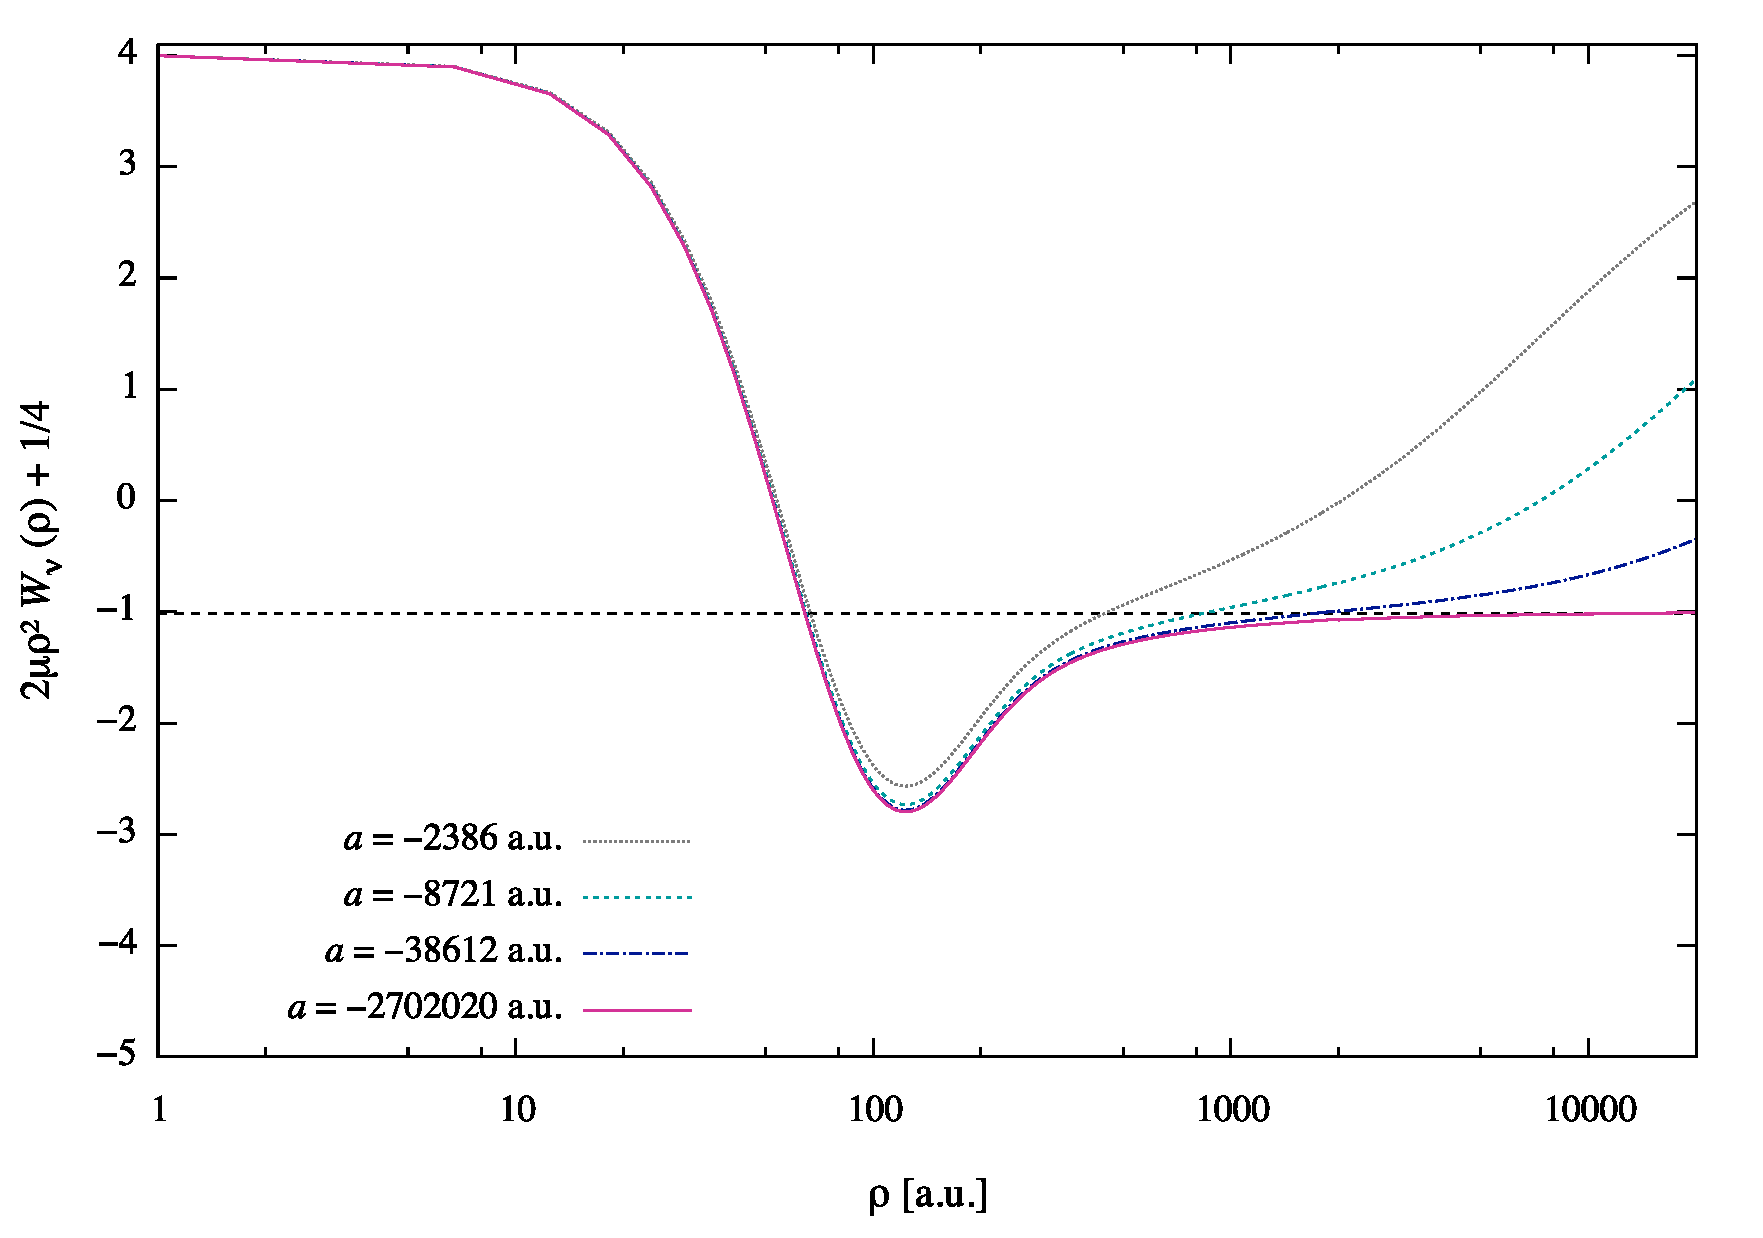
\includegraphics[width=0.8\linewidth]{finite_negative_a.pdf}
	\end{figure}
\end{figure}
\end{frame}


%----------------------------------------------------------------------------------------

\end{document} 